\subsection{Benchmark}
Student clearly defines a benchmark result or threshold for comparing performances of solutions obtained.

For the CNNs architecture, it is quite important to decide the number of layers.Therefore, I first choose several convolutional layers and decide one of them as a benchmark.

When deciding the architecture, I set the mutual parameters as follows.
The number of batch size is 32.The number of filters of each convolutional layer is 32. and finally the number of epochs is 20.

I tried 4 architecture of CNNs.

\begin{enumerate}
 \item 1 Convolutional layer \& 2 Fully connected layers \\
 The simplest version in these model.The input and output dimension on each layer are below.
 The accuracy rate of training and validation data are also below.
 
 \begin{figure}[H]

	\begin{center}
	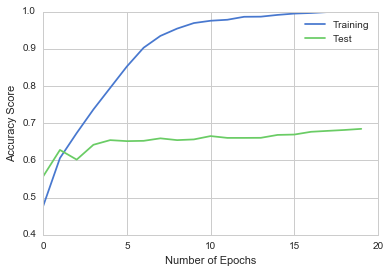
\includegraphics[width=5cm]{picture/1layer_cnn.png}
	\caption{Accuracy rate of training and validation data}
	\end{center}
	\label{fig:eight}

\end{figure}
 
 The accuracy rate on the training data is quite high,however the accuracy rate on the validation data is low. This means that this architecture falls into over-fitting.
 
 
 \item 2 Convolutional layers \& 2 Fully connected layers \\
 The input and output dimension on each layer are below.
 The accuracy rate of training and validation data are also below.
 
 \begin{figure}[H]

	\begin{center}
	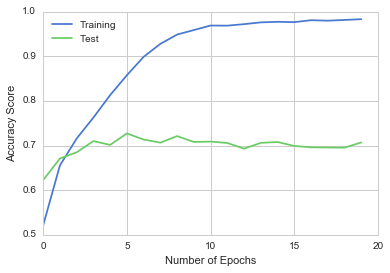
\includegraphics[width=5cm]{picture/2layer_cnn.png}
	\caption{Accuracy rate of training and validation data}
	\end{center}
	\label{fig:nine}

\end{figure}

This architecture also caused over-fitting as mentioned above.

 \item 3 Convolutional layers \& 2 Fully connected layers \\
 The accuracy rate of training and validation data are also below.
 
 \begin{figure}[H]

	\begin{center}
	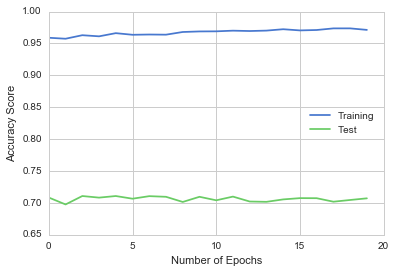
\includegraphics[width=5cm]{picture/3layer_cnn.png}
	\caption{Accuracy rate of training and validation data}
	\end{center}
	\label{fig:ten}

This architecture also falls into over-fitting.

\end{figure}
 \item 4 Convolutional layers \& 2 Fully connected layers \\
 The accuracy rate of training and validation data are also below.
 
 \begin{figure}[H]

	\begin{center}
	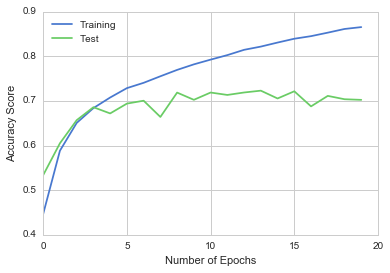
\includegraphics[width=5cm]{picture/4layer_cnn.png}
	\caption{Accuracy rate of training and validation data}
	\end{center}
	\label{fig:eleven}

\end{figure}
\end{enumerate}


This architecture is far better than the others. The accuracy rate of both training and validation data is high as the number of epochs increases.
The accuracy rate of this architecture is 70.2\%. Actually the highest accuracy rate in CIFAR-10 is more than 95.0\% and the benchmark is quite lower than the highest one. My target in this task is to find the optimal parameters for the architecture. Therefore, I'll utilize this 4 layers convolution \& 2 fully connected layers architecture as a benchmark.


From these results, I choose the fourth architecture(4 convolution layers \& 2 fully connected layers) as the benchmark for this task.
